%%%%%%%%%%%%%%%%%%%%%%%%%%%%%%%%%%%%%%%%%%%%%%%%%%%%%%%%%%%%%%%%%%%%%%
% How to use writeLaTeX: 
%
% You edit the source code here on the left, and the preview on the
% right shows you the result within a few seconds.
%
% Bookmark this page and share the URL with your co-authors. They can
% edit at the same time!
%
% You can upload figures, bibliographies, custom classes and
% styles using the files menu.
%
%%%%%%%%%%%%%%%%%%%%%%%%%%%%%%%%%%%%%%%%%%%%%%%%%%%%%%%%%%%%%%%%%%%%%%

\documentclass[12pt]{article}
%\documentclass[]{interact}
\usepackage{sbc-template}
\usepackage[round]{natbib}
\usepackage{amsmath}
%\usepackage{booktabs}
\usepackage{color,soul}
\usepackage{graphicx,url}
\usepackage{multicol}
\usepackage{diagbox}
\usepackage[dvipsnames]{xcolor}
\usepackage{verbatim}
\usepackage{makecell}

\newcommand{\R}[1]{~\scriptsize{(#1)}}
\newtheorem{definition}{Definition}
% Keywords command
\providecommand{\keywords}[1]
{
  \small    
  \textbf{\textit{Keywords---}} #1
}


%\usepackage[brazil]{babel}   
\usepackage[utf8]{inputenc}  

     
\sloppy

%\title{SMSM: a Similarity Measure for Trajectory Stops and Moves}
%\author{Andre L. Lehmann\inst{1}, Luis Otavio Alvares\inst{1}, Vania Bogorny\inst{1} }


%\address{Programa de Pós-Graduação em Ciência da Computação \\Departamento de Informatica e Estatistica, Universidade Federal de Santa Catarina\\ Florianopolis, Santa Catarina, Brasil
%  \email{andre.lehmann@posgrad.ufsc.br,alvares@inf.ufsc.br ,vania.bogorny@ufsc.br}
%}

\begin{document} 

%\maketitle

% \begin{abstract}
% For many years trajectory similarity research has focused on raw trajectories, considering only space and time information. With the trajectory semantic enrichment emerged the need for similarity measures that support space, time, and semantics. Although some trajectory similarity measures deal with all these dimensions, they consider only stops, ignoring the moves. We claim that, for some applications, the movement between stops is as important as the stops, and they must be considered in the similarity analysis.
%   In this article we propose SMSM, a novel similarity measure for semantic trajectories that considers both stops and moves.
%   SMSM is evaluated with real trajectory data of CRAWDAD and Geolife. The results show that SMSM overcomes state-of-the-art measures developed for both raw and semantic trajectories.
% \end{abstract}

%\keywords{Trajectory similarity measures, semantic trajectory similarity}

\section{Introduction}
%--vania revisando
Trajectory similarity measuring has received significant attention in the last few years, and several measures have been proposed \hl{to deal either with raw trajectories or semantic trajectories}. A \emph{raw trajectory} is generally represented as a sequence of points $T=<p_1, p_2, ...p_n>$, with $p_i=(x_i,y_i,t_i)$ where $x,y$ is the position of the object in space at time instant $t$.  Examples of similarity measures for raw trajectories are LCSS (Longest Common SubSequence) \citep{vlachos2002discovering}, EDR (Edit Distance on Real sequences) \citep{Chen:2005:RFS:1066157.1066213}, NWED (Normalized Weighted Edit Distance) \citep{dodge2012} and UMS (Uncertain Movement Similarity) \citep{Furtado-UMS-2018}. LCSS \citep{vlachos2002discovering} and EDR \citep{Chen:2005:RFS:1066157.1066213}, developed for raw trajectories, consider the sequence of elements, but they force a match in all dimensions, not allowing partial similarity between trajectory elements.  %\hl{Multi-Dimensional Dynamic Time-Warping} (MD-DTW) \cite{ten2007multi} is another approach that is able to handle multiple dimensions. It extends \hl{Dynamic Time-Warping} (DTW) \cite{berndt1994using} in order to find the distance between two sequences by looking for the best contiguous match of elements according to the sum of the distances in all dimensions. The problem of DTW and MD-DTW is that they consider the real distance between the elements, are sensitive to noise, and were developed for numerical attributes, not dealing with semantic information. 
UMS \citep{Furtado-UMS-2018} is a parameter free method that considers only the spatial dimension, but it outperformed all previous works for raw trajectory similarity.


Existing works for raw trajectory similarity are limited to the spatio-temporal properties of raw trajectories, basically considering trajectories as objects with only space information or space and time.

In 2008, emerged the concept of semantic trajectories \citep{Spaccapietra:2008:CVT:1347466.1347785}, where trajectories are represented as \emph{sequences of stops and moves}. \emph{Stops} are the most important parts of trajectories, representing the places that an object has visited for a minimal amount of time, and the \emph{moves} are the trajectory points between stops. In several works, stops are called points of interest (POIs), episodes, or stay points. Semantic trajectories are more complex than raw trajectories, because they have at least three dimensions: space, time, and semantics. \textcolor{red}{We consider in this paper that semantics is any type of information associated to mobility data other than spatial location and time.}

\textcolor{red}{The enrichment of trajectories with semantic information is a well studied topic in the literature, and a number of methods have been proposed to semantically enrich trajectories, as the works of} \cite{alvares2007model}, \cite{Palma2008}, \cite{manso}, and \cite{fileto2013baquara}. \textcolor{red}{Examples of semantic information related to the stops can be, for instance, the name of the stop (e.g. Ibis Hotel) and the category (e.g. Hotel, Museum, Restaurant), while the semantic information related to the move could be, for instance, the name of the streets followed by the moving object and the category of the transportation mean. The explosion of social media data, internet channels, and the facility to enrich trajectories with more context information as linked open data, allow the representation of movement in a more meaningful way. From social media data, for instance, a stop at a hotel can be enriched with the information of the number of stars, the price average, evaluation rate, facilities, parking, wifi, etc.  In this paper we assume that semantic trajectories are represented as sequences of stops and moves, as originally defined in \cite{Spaccapietra:2008:CVT:1347466.1347785} and the way how these trajectories are generated or enriched is out of the scope of this paper. }

\textcolor{red}{Only a few  similarity measures were proposed for semantic trajectories, as \cite{Kang:2009:SMT:1529282.1529580}, \cite{Liu:2012:SMM:2442968.2442971}, \cite{Ying:2010:MUS:1867699.1867703}, \cite{Furtado:TGIS12156}. The main problems of these measures is that they do not address all three dimensions (space, time and semantics), as the works of \cite{Kang:2009:SMT:1529282.1529580} and \cite{Liu:2012:SMM:2442968.2442971}; or, 
they exclusively address the stops, systematically ignoring all information about the moves, as the works of \cite{Ying:2010:MUS:1867699.1867703} and \cite{Furtado:TGIS12156}. To the best of our knowledge, none of the existing similarity measures for semantic trajectories have considered both stops and moves.} The measure MSM (Multidimensional Similarity Measure) \citep{Furtado:TGIS12156}, for instance, considers only the stops, and they are treated as elements that are independent from each other, without considering the order/sequence as they appear in the trajectories. \textcolor{red}{ MSM can answer questions like: \emph{how similar are two trajectories $P$ and $Q$ considering their stops?} For the three tourist trajectories shown in Figure \ref{fig:Paris} that visit four places in Paris, MSM would give a similarity degree of 100\%, since they visited the same stops.}

 

\textcolor{red}{Similarity measures are the basis of several data processing and analysis techniques, such as information retrieval, location prediction, nearest neighbour queries, outlier detection, clustering, etc. A clustering algorithm, for instance, uses a similarity measure for grouping objects with similar trajectories. Outlier detection methods use similarity to find groups of trajectories with normal behavior, and the objects that are dissimilar to the majority, are the outliers. \textcolor{blue}{To detect specific trajectory patterns such as flocks \citep{Laube2005}, for instance, the similarity of spatial features can be used to find the objects moving together}. Similarity measures that consider both stops and moves can be important in a vast number of application such as public transportation systems, traffic management, fraud detection, tourism, etc. }
%To mention a few examples, similarity measures are the basis for finding objects that follow the same routes, tourists that visit similar places at similar times, to distinguish categories of users such as students from professors at a university, to find similar taxi trajectories, to find users that use the same means of transportation when visiting the same places, etc.


\begin{figure}[h]
\label{fig:Paris}
\centering
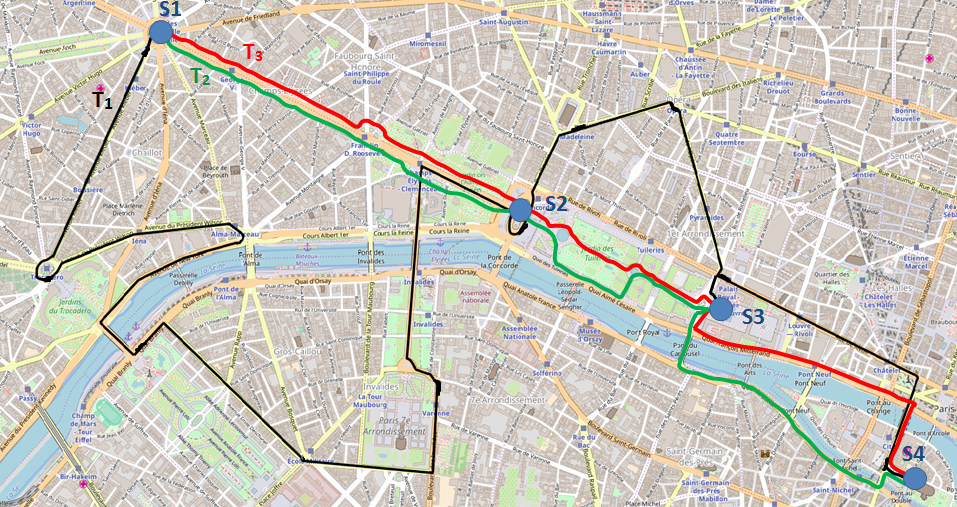
\includegraphics[width=1.0\textwidth]{Images/paris4.png}
\caption{Tourist trajectories in Paris with four stops}
\end{figure}


\textcolor{red}{To better understand the need for considering both stops and moves in trajectory similarity analysis, let us consider the example in Figure \ref{fig:Paris}, for a tourism application, where we have three trajectories of tourists visiting Paris. These tourists visited four places, in this order:  Arc de Triomphe (first stop - S1), Place de la Concorde (second stop - S2), the Louvre Museum (third stop - S3), and the Notre Dame Cathedral (the last stop - S4). The three tourists visited the same places at the same order, but the tourists of trajectories $T2$ (green trajectory) and $T3$ (red trajectory) moved on foot, following the shortest path, while the tourist of trajectory $T1$ used a city tour hop on and hop off bus to appreciate the view. The question we want to answer is \emph{how similar are trajectories T1, T2 and T3 considering both stops and moves?} From the figure it is clear that trajectories T1 and T2 are more similar, because they used almost the same paths between stops, while trajectory T3 has a completely different move. Now suppose that a tourism manager wants to recommend a trip to a new tourist arriving in Paris, but he has a time constraint to stay from 9AM to 4PM, and he wants to visit the same places visited by the tourists in the figure. From the whole database of trajectories, a query must return the most similar trajectories to the trajectory that this new user wants to perform. It is clear that for this problem, a good recommendation is only possible if we consider the sequence of visited places, the duration of the visits, the real path followed during the move, as well as the move transportation mode. \hl{ mas nesse exemplo nao tem como informar o move, para buscar os mais similares. O sistema de  recomendacao faria a recuperacao  baseado apenas nos stops e no tempo total gasto} The measure MSM would not distinguish the trajectories in Figure 1, giving a 100\% similarity. Other measures as UMS, EDR, and LCSS would not consider the visited places, only the raw trajectories, so they would not be able to retrieve trajectories that visited the given places and the moves performed between the places.
}

 \textcolor{red}{In trajectory fraud detection, for instance, a taxi fraud trajectory, which is an outlier in relation to the majority of taxi trajectories between two regions of interest, a similarity measure must be able to consider the start and end stop of a trip to find the group of normal trajectories, which are supposed to follow the closest or fastest path, while the outlier trajectory will be the one where the driver made a longer trip. A real example of an outlier taxi trajectory is shown in Figure \ref{fig:crawdad_outlier}, extracted from the San Francisco dataset of the Crawdad project} \citep{epfl-mobility-20090224}.
 
\begin{figure}[h]
\centering
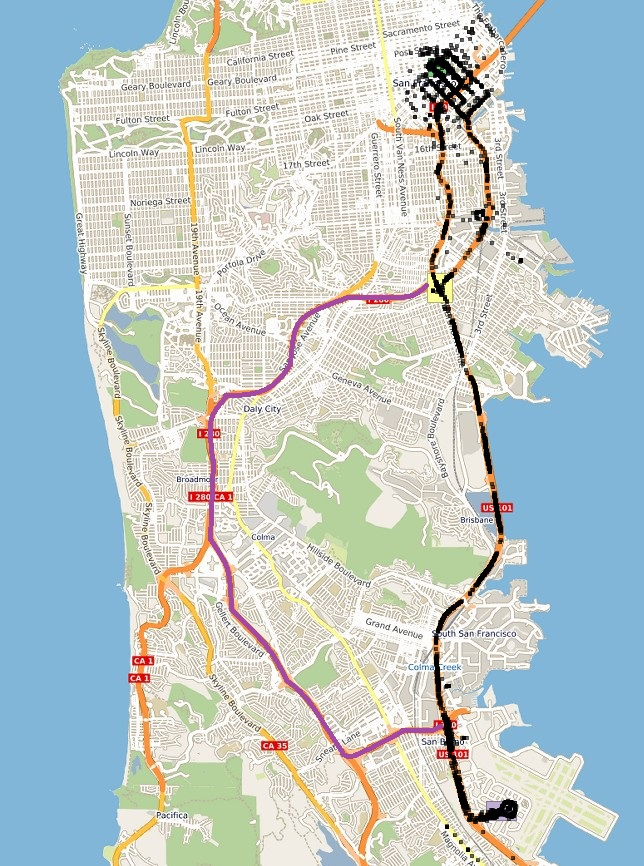
\includegraphics[width=0.5\textwidth]{Images/CRAWDAD-Outlier.jpg}
\caption{\label{fig:crawdad_outlier} An outlier trajectory (in purple) going from Airport to downtown of San Francisco}
\end{figure}

\hl{Nao seria melhor ficarmos soh com os outros dois cenarios?}
\textcolor{red}{Another real application where the similarity of stops and moves is necessary is a sales promoter domain. In a sales promoter application, the company wants the employee to visit several places during one day, and wants to maximize the visits at the stops and minimize the duration of the moves. In order to find the most optimized trajectory of an employee, it is necessary to consider the sequence of the stops, the duration of the stops, the path followed during the moves and the duration of the moves. In order to automatically detect the best trajectory of each promoter among a set of trajectories, it is necessary to use both stops and moves.} \hl{FOCAR MAIS NA SIMILARIDADE}
 

%We claim that for several applications, the moves are as important as the stops, or even more important. Moves carry important information such as the traveled distance from one place to another, the transportation means, the name of the streets followed by the moving object, the average speed, etc. Moves are important for answering semantic queries that involve both stops and moves such as (i) which objects go from a stop A (e.g. city center) to a stop B (e.g. airport) through the same roads? Which is the most popular route from A (e.g. city center) to B (e.g. University x)?}

%Answering this kind of question is important in several applications. In car sharing systems, for instance, the origin and destination of the trip is important, but the path followed between the origin and destination is important as well, in order to find ride intersection. In public transportation systems, both bus stops and streets must be known to propose new bus lines. In traffic management applications, the moves between spatial regions must be used to detect traffic jams.


In this paper we propose a new semantic trajectory similarity measure that extends MSM, proposed in \cite{Furtado:TGIS12156}, to support both stops and moves. Our approach considers the sequence of the stops, what is not supported by MSM, and allows different semantics for the moves. 
In summary, we make the following contributions:
(i) we propose a new similarity measure for multidimensional sequences treating elements with heterogeneous dimensions, which is the case of stops and moves; (ii) the semantic similarity measure considers both \textit{stops} and \textit{moves}, as well as their space, time, and semantic dimensions, allowing the use of different distance functions for each dimension; (iii) the measure is flexible enough to consider the order between stops, ignore the moves when it is the case for the application, and supports different weights for stops, moves, and dimensions, allowing to give more importance to stops, moves, or data dimensions; (iv) we evaluate the proposed measure with experiments over real data, comparing our proposal to both semantic and raw trajectory similarity measures.

The rest of this article is organized as follows: Section \ref{sec:related} presents the related works, Section \ref{sec:proposed_measure} presents the proposed similarity measure with a running example, Section \ref{sec:experiments} presents experiments over real trajectory data, and Section \ref{sec:conclusions} concludes the article.

%\hl{Similarity measures play a important role in geospatial information systems, as a tool to analyze the closeness of elements. As an example, we can use a public transportation system. To define a creation of a new bus stop some characteristics should be analyzed: (i) the current usage rate of the bus line; (ii) the growth of population in the region; (iii) the usage rate of alternatives transportation means, as car-pooling systems and taxis; (iv) the size and count of important community buildings, as schools, hospitals, public administrative buildings, etc. So, if a bus line has as characteristic a lower usage rate and near of it occurs a higher usage of other transportation means as car-pooling or taxi, it is expected that the creation of a bus stop will rise the usage rate of buses at the expense of car use. It can reduce traffic jams in the region, it may reduce the air pollution in the city, in addition of being more financially advantageous for passengers. But to define exactly where the bus stops should be created, first of all it is necessary to find out which bus lines cover the region and which are the bus stops shared between them. We use the bus stops as the \emph{stops} and the street names as the \emph{moves} in the stop and move model. After modeling our semantic trajectories, we can find the best place to put a new bus stop by finding a \emph{move} which can be split in two segments, creating a \emph{stop} (the new bus stop) between them. If this new simulated trajectory is more similar to original trajectories, it indicates that the bus line will be slightly changed, having little impact on the mesh of bus lines as a whole.}




\section{Related works} \label{sec:related}
Along the last years, many similarity measures for trajectories were proposed focused on raw trajectories, which find the similarity between two trajectories using only trajectory raw data, as spatial and temporal information. Vlachos in \cite{vlachos2002discovering} proposed the LCSS \hl{(Longest Common SubSequence)} for raw trajectories. In this work two points \textit{match} when the distance between them is less than a given threshold. The longer the common subsequence of matches between two trajectories, the more similar they are. Chen in \cite{Chen:2005:RFS:1066157.1066213} proposes the EDR \hl{(Edit Distance on Real sequences)}, another similarity measure for raw trajectory data that calculates the edition difference between the points, as classical edit distance measures. Another measure of similarity for raw trajectories is \hl{w-constrained discrete Frechet distance} (wDF), proposed in \cite{Ding:2008:ESJ:1440463.1440989}. wDF can not deal with dimensions other than space, limiting it to raw trajectories. Although LCSS and EDR have not been proposed for this intent, both measures can be easily extended to handle other dimensions (e.g. semantics). However, that extensibility does not allow the measures to represent semantic trajectories as a sequence of heterogeneous elements, that is the case of stops and moves, because both LCSS and EDR demand that all trajectory elements should be homogeneous.

\textcolor{red}{UMS was proposed in \cite{Furtado-UMS-2018} as a new parameter-free similarity measure for raw trajectories. UMS was designed exclusively for raw trajectories, considering only the spatial dimension. The major contribution of UMS is that no distance threshold is needed, and the distance between two trajectories is computed with ellipses over every two trajectory points, so trajectories are represented as sequences of ellipses. The similarity is given by the proportion of ellipse intersection. As the ellipses are dynamically defined based on point distance, UMS solves the problem of trajectories with distinct or varied sampling rates, by computing each ellipse size as big as necessary to cover two consecutive points. UMS outperformed all state-of-the-art works for raw trajectories developed before 2018, so it is currently the best similarity measure for raw trajectories.}

%\hl{Distinctly of the raw points measures, in the work of }\cite{Laube2005}\hl{ a raw trajectory is analyzed through the derived features of the movement, such as speed changing, momentous speed and others. The main purpose of work of Laube is to define a few behavior patterns in raw trajectories and find spatial encounters in respect to these behaviors. Using the REMO concept (RElative MOtion), it approach has as constraint that analyzed trajectories must be synchronized in time. This is not the case in real life trajectories of persons or regular vehicles, since each moving object (person, vehicles, etc) starts its movement independently each other, limiting it uses for some specific contexts, such as birds migration, wildlife monitoring, etc. In a similar way, the work proposed in } \cite{Shirabe2006}\hl{ shows that a strong correlation of motion features can help to find a linear correlation between trajectories in raw trajectory datasets. A drawback of the approach is the inability to consider the spatial and temporal location of each point. In other words, the trajectories are analyzed only by their behavior and not by their discrete points.}

The Common Visit Time Interval (CVTI) is proposed in \cite{Kang:2009:SMT:1529282.1529580} as a measure to integrate the semantic dimension of the stops with the temporal dimension. Although using different data dimensions, the measure is not extensible for other dimensions associated with the point, not allowing heterogeneous data such as stops and moves to be modeled and measured together.

In \cite{Ying:2010:MUS:1867699.1867703} the measure \hl{Maximal Semantic Trajectory Pattern} (MSTP) is proposed, which despite being a measure for semantic trajectories is not able to handle multiple data dimensions. Moreover, as MSTP essentially works with the frequency at which stops are visited, it is not able to represent moves between stops, ignoring all information about the movement between the stops.

The distance measure Dynamic Time-Warping adaptive (DTWa) proposed in \cite{Shokoohi-Yekta2017} extends the classical \hl{Dynamic Time-Warping} (DTW) \cite{berndt1994using} distance measure by allowing two data series to have their distance measured using multiple data dimensions. The input of DTWa must be a sequence of points with homogeneous dimensions, so having similar problems as previous measures.

In the work of \cite{Furtado:TGIS12156}, the MSM measure is proposed, working with multiple dimensions. In MSM all elements must be homogeneous, not allowing the representation of heterogeneous elements as stops and moves. MSM is more robust than LCSS and EDR by allowing partial dimension match and not forcing a sequence. MSM was developed to work only with stops, and the sequence of elements is not taken into account during the similarity calculation, ignoring the order of the stops. We claim that for some applications as car sharing, new bus route planning, and traffic analysis, the sequence of stops plays an essential role.

%=====================================================================================
%======================================================================================


\section{The Proposed Measure: SMSM} \label{sec:proposed_measure}
In this section we present a novel similarity measure to consider both stops and moves of semantic trajectories, called SMSM (\textit{Stops and Moves Similarity Measure}). The idea behind SMSM is a measure that overcomes the strictness of LCSS and EDR by allowing partial order and dimension matching, and the limitations of MSM by considering both stops and moves. Before we introduce the concepts related to the new measure, we formally define semantic trajectory, considering its sequence of stops and moves, which is an enriched extension of the definition presented in \cite{Spaccapietra:2008:CVT:1347466.1347785}:


\begin{definition}
\label{def:semantic_trajectory}
A semantic trajectory  $ST=\langle s_1, m_1, s_2, m_2, s_3,m_3, ...., s_n, m_n, s_{n+1} \rangle$ is a time ordered sequence of stops and moves, where each stop $s_i$ has a set of attributes $\{d_{s1}, d_{s2}, ...d_{sq}\}$ characterizing it according to q-dimensions, and each move $m_j$  has a set of attributes $\{d_{m1}, d_{m2}, ...d_{mr}\}$  characterizing it according to r-dimensions. 
\end{definition}

In this work we assume that a semantic trajectory starts and ends with a stop, otherwise we transform the first and/or the last point of the trajectory in a stop. In the following section we present the new concepts and the definition of the proposed similarity measure SMSM.
\subsection{Basic Concepts and the Proposed Measure}

Stops and moves by definition are different and heterogeneous trajectory elements. A stop may have a spatial position, a start and end time, a category, or a set of attributes related to the category (e.g. Category hotel, stars, rate, price), etc. A move always starts and ends in a stop and may be characterized by different attributes as average speed, traveled distance, sequence of streets, duration, the sequence of raw points, etc. These attributes are defined according to the needs of the application. 

In order to deal with these heterogeneous elements (stops and moves), we introduce the concept of \emph{movement element}. A movement element is a new representation that is not treated by other measures, mainly MSM, which supports only stops. Indeed, MSM does not consider the order of trajectory elements, while in our approach we preserve the sequence of both stops and moves in a movement element.

\begin{definition}
\label{def:movement_element}
A movement element  $e=(stopS, move, stopE)$ is a tuple formed by a start stop $stopS$, the $move$ between $stopS$ and  $stopE$, and the end stop $stopE$, where stopS and stopE are two consecutive stops.
\end{definition}


Hereafter we will consider a semantic trajectory as a sequence of \textit{homogeneous movement elements}, as follows: 
$ST=\langle e_1=(s_1,m_1,s_2), e_2=(s_2,m_2,s_3), ..., e_n=(s_n,m_n,s_{n+1}) \rangle$.

Notice that we define a movement element as a homogeneous trajectory part, but they will be analyzed separately later in our measure.
This structure will be used for the proposed similarity measure, where one trajectory will be compared with another one based on their movement elements.



We analyze the similarity of a movement element $a\in A$ with another movement element $b\in B$, where A and B are semantic trajectories, in two parts: their stops and their moves.The basis for measuring the similarity of these two parts is the \emph{match} function, given in Equation \ref{func:match1}. The function returns 1 if the distance between an attribute (also called dimension) of two movement elements is less than a given threshold \emph{maxDist}, and zero otherwise. This function is used for measuring the distance of all dimensions of both: the stops and the moves.

\begin{equation}
%\scriptsize
\label{func:match1}
  match_i(a, b) = 
  \begin{cases} 
      1 & dist_i(a, b) \leq maxDist_i \\
      0 & otherwise
  \end{cases}
\end{equation}

To compute a total score for two movement elements $a$ and $b$ we define the function \emph{score(a,b)} in Equation \ref{func:score1}, where, $w_{stop}$ and $w_{move}$ are the weights of the stops and the moves, respectively, and their sum should be one. The importance of either stops or moves can vary from one application to another, so we can use the weights to give the respective importance. 


\begin{equation}
%\scriptsize
\label{func:score1}
score(a, b) = scoreStop(a, b) * w_{stop} + scoreMove(a, b) * w_{move}  
\end{equation}


In our measure we consider a score for the stops (scoreStop) and a score for the move (scoreMove). The functions \emph{scoreStop(a,b)} and \emph{scoreMove(a,b)} are defined in Equations \ref{func:scoreStop1} and \ref{func:scoreMove2}, respectively. In both equations, $r$ and $q$ are the number of dimensions (attributes) of stops and moves, respectively. The score of the stops, computed according to Equation \ref{func:scoreStop1}, is given by the average of all dimension matches of the start and end stops of two movement elements $a$ and $b$. 


\begin{equation}
%\scriptsize
\label{func:scoreStop1}
%\begin{split}
  scoreStop(a, b) = \sum\limits_{i=1}^r (match_i(a_{stopS}, b_{stopS}) + match_i(a_{stopE}, b_{stopE}))\div 2* w_{i}
%\end{split}
\end{equation}


\begin{equation}
%\scriptsize
\label{func:scoreMove2}
\begin{split}
scoreMove(a, b)  & = 
  \begin{cases} 
      \sum\limits_{i=1}^q match_i(a_{move}, b_{move}) * w_{i} & if matchStops(a, b)\\
      0 & otherwise
  \end{cases}
\end{split}
\end{equation}


%The sum of the weights in Equations \ref{func:scoreStop1} and \ref{func:scoreMove2} should be one.
Note in Equation \ref{func:scoreMove2} that the \emph{scoreMove} depends on the function \textit{matchStops(a, b)}. \textcolor{red}{The intuition is that two moves should be evaluated only if their starting positions (starting stops) are spatially close and the ending positions (ending stops) are close as well.}
    The function \emph{matchStops(a,b)} is true when the \hl{spatial distance} between $a_{stopS}$ and $b_{stopS}$  as well as between $a_{stopE}$ and $b_{stopE}$ is less than $maxDist$.
    
    %\textcolor{red}{In real scenarios, this means that if we want to analyze movement elements, for instance, from France to Italy, we do not need to compare these trajectories with others moving from France to Spain, since the ending stop is different}.

\textcolor{blue}{Figure \ref{fig:move} shows an example of four movement elements representing part of four trajectories. The movement elements are $<A, P_1, B>$, $<A, P_2, B>$, $<A, P_3, B>$ and $<A, P_4, C>$, where $A$, $B$, and $C$ are the stops, and $P$ are the moves. The function \emph{scoreMove} will analyze only the moves of the movement elements that have $A$ as the start stop and $B$ as the end stop, so the moves $P_1, P_2, P_3$. 
%So the \emph{moves} of the movement elements $<A, P_1, B>$, $<A, P_2, B>$, $<A, P_3, B>$ will be analyzed because they have the same start and end stop.}
The movement element $<A, P_4, C>$ will not have a score for the move because if compared to the other three movement elements, only the start stop has a match, and as the end stops does not match, the move $P_4$ will not be analyzed.}

 %and three trajectories move to $B$ following three different paths.  In the example in Figure \ref{fig:move}, if we are interested in trajectories moving from A to B, our measure will only analyze the moves $P1$, $P2$, and $P3$ of trajectories going from A to B, and these three moves will not be compared with $P4$. 

%\hl{Differences among the three movement elements rely exclusively on the differences of the move. On the other hand, the difference of these movement elements to movement element $<A, P_4, C>$ is more evident, since if it end stop is distinct, the move is distinct too. Based on this, SMSM do not compare the move of $<A, P_4, C>$ with the others movement element.}

\textcolor{blue}{The function \emph{scoreMove} guarantees a partial order in the similarity analysis, what has not been considered by MSM, which is the closest measure to our approach, but that considers only stops and without any order. Considering that the four movement elements in Figure \ref{fig:move} belong to four different trajectories, MSM would give the same similarity for the parts of the trajectories going from $A$ to $B$, because it does not look the moves, and 50\% similarity with the trajectory going from $A$ to $C$ because they share 50\% of the stops.
}\textcolor{green}{If we consider the example in the figure as a real scenario, where $A$, $B$, and $C$ represent  places as France, Italy, and Spain, respectively, we believe that the three trajectories going from France ($A$) to Italy ($B$) must have their move analyzed because they visit the same sequence of places, while the trajectory that goes from France ($A$) to Spain ($C$) does not share the same destination, so the move of this trajectory is not considered in the analysis.}



\begin{figure}[h]
\centering
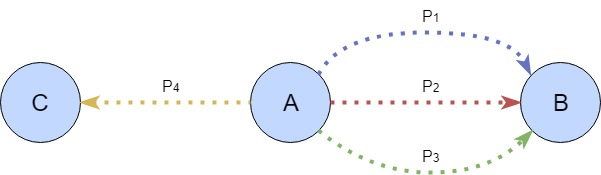
\includegraphics[width=0.75\textwidth]{Images/Toy_trajectories.jpg}
\caption{\label{fig:move} Movement elements: stop $A$ to stop $B$ with the moves $P_1$, $P_2$, and $P_3$; and Movement element: $A$ to $C$ with the move $P_4$}
\end{figure}

Having defined the score for stops and moves for comparing movement elements, Equation \ref{func:parity} defines the parity of two semantic trajectories $A$ and $B$. The parity of $A$ with $B$ is the sum of the highest score of all the elements $a \in A$ when compared with all the elements of $B$.
\begin{equation}
\label{func:parity}
parity(A, B) = \sum\limits_{a\in A} \textbf{max}\{\textit{score}(a, b) : b \in B\}
\end{equation}

Finally, we can define the global similarity of two trajectories $A$ and $B$ with $SMSM$. Equation \ref{func:SMSM1} defines the stops and moves similarity measure $SMSM(A,B)$ by the average parity of $A$ with $B$ and of $B$ with $A$. \hl{The average parity is given by the sum of both parities over the sum of the number of elements in $A$ ($|A|$) and the number of elements in $B$ ($|B|$).}

\begin{equation}
\label{func:SMSM1}
%\scriptsize
\begin{split}
  SMSM(A, B) = 
  \begin{cases} 
      0 & if  |A| = 0 \vee |B| = 0 \\
      \frac{parity(A, B) + parity(B, A)}{|A| + |B|} & otherwise
  \end{cases}
\end{split}
\end{equation}



\subsection{Evaluation over a running example}

In this section we present a running example, comparing SMSM and MSM, since MSM is the closest approach to the proposed similarity measure.
Let us consider the two trajectories shown in Figure \ref{fig:bus}. Trajectory $Q$ represents the daily routine of a professor, that starts his day at the gym in the morning, while trajectory $P$ is the daily routine of a student, that starts his day at a coffee shop. The trajectories are annotated with the stop category, start and end time of the stop, an hypothetical geographic position, spatial position of the stop and the main street followed during the moves. So considering the \hl{notation \textit{stop name ((spatial position x, spatial position y), [start timestamp - end timestamp])}}, the student has the following movement behavior: stays at \textit{Home} $((96,215), [8pm-8am])$, \hl{then} he goes via Edu Vieira street to have breakfast at the \textit{Coffee shop} $((182,201), [8:50am-10am])$, and from there goes via Delfino Conti street to the \textit{University} $((59,127), [10:25am-6:10pm])$, finishing the day moving via Henrique Fontes street to the \textit{Gym} $((268,63), [7:30pm-9pm])$. The professor (trajectory $Q$) goes from \textit{Home} $((13,81), [7pm-7am])$ via Beira-mar avenue jogging at the \textit{Gym} $((268,63), [7:30am-8:30am])$. After he goes to the \textit{Coffee shop} $((182,201), [8:45am-9:55am])$ via Edu Vieira street, and via Delfino Conti reaches the \textit{University} $((59,127), [10:15am-7:45pm])$ to teach his classes until the end of the day. We have two trajectories $P$ and $Q$ with their stops and moves annotated with the category of the place, the spatial information of the visited place, the time of the visit, and the name of the street to represent the move. Both trajectories visit the same places, sharing some streets, but in totally different order.
\begin{figure}[h!]
\centering
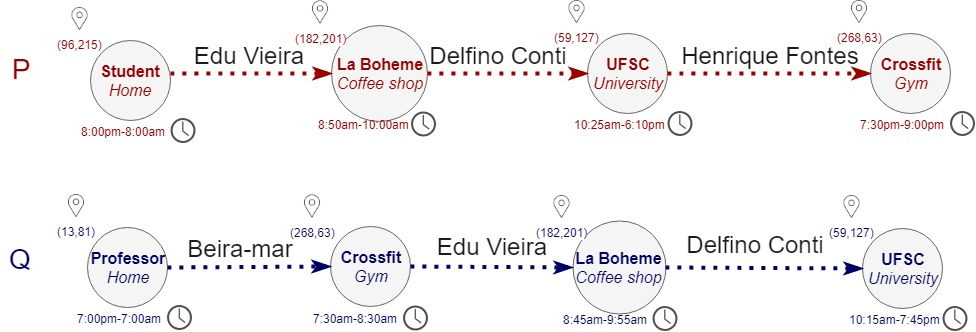
\includegraphics[width=1\textwidth]{Images/running_example.jpg}
\caption{\label{fig:bus} Semantic Trajectories $P$ (Student) and $Q$ (Professor) with stops and moves}
\end{figure}


In order to calculate the SMSM similarity value, we first need to construct all movement elements for each trajectory. Table \ref{tab:SMSM_tuples} lists these elements, where each element contains the start stop, the name of the street followed during the move, and the next stop. Notice in this table that the only movement element where the moves will be measured is $<Coffee shop, Delfino Conti, University>$ from trajectory $P$ and $<Coffee shop, Delfino Conti, University>$ from trajectory $Q$, because both start and end stops match.

\begin{table}[h!]
\scriptsize
  \centering
  \begin{tabular}{|c|c|}
  	\hline
		\textcolor{Red}{\textbf{Student (P)}} & \textcolor{Blue}{\textbf{Professor (Q)}}\\
  	\hline
      $<$Home, Edu Vieira, Coffee$>$&$<$Home, Beira-mar, Gym$>$\\
      $<$Coffee, Delfino Conti, University$>$&$<$Gym, Edu Vieira, Coffee$>$\\
      $<$University, Henrique Fontes, Gym$>$&$<$Coffee, Delfino Conti, University$>$\\
  	\hline
  \end{tabular}
  \label{tab:wrong}
  \caption{Movement elements}
  \label{tab:SMSM_tuples}
\end{table}

To measure the distance between two movement elements, we use the following functions for measuring the distance of each stop dimensions: 
\begin{itemize}
  \item Space: the Euclidean distance between the centroids of the stops;
  \item Time: let $[t1, t2]$ be the time interval of a stop. The time distance of two stops is given by:
\begin{equation} \label{eq:time_interval}
	dist_t(a, b) = 1 - \dfrac{duration([a.t1, a.t2] \cap [b.t1, b.t2])}{duration([min(a.t1, b.t1), max(a.t2, b.t2)])}
\end{equation}
  \item Semantics: the distance is equal to 0 in case of exact match and equal to 1 otherwise.
\end{itemize}

For the sake of simplicity, for the move, in this example we consider only the semantic information, i.e., the name of the followed street, where the distance is equal to 0 in case of exact match of street name and equal to 1 otherwise.

In this running example we use as thresholds \textit{maxDist\textsubscript{space}} = 100 meters and \textit{maxDist\textsubscript{time}} = 0.5, i.e. two stops are said as matched in time when both share half of their period in that stop.
With distance functions and threshold values defined and elements constructed, we use Equation \ref{func:score1} to measure the similarity values between all element dimensions, computing first the match in both start and end stops and if the stops match we compute the match for the move. 

To understand how to measure the movement element similarity let us consider the movement elements $element_{P}=<Home_{[8pm-8am]},Edu Vieira,Coffee shop_{[8:50am-10am]}>$ and $element_{Q}=<Home_{[7pm-7am]},Beira-mar,Gym_{[7:30am-8:30am]}>$. First, we apply the function $match()$ (Equation \ref{func:match1}) for the stops. In this case, the start stops have some degree of similarity: their semantics is the same and the time distance of $Home_{P}$ and $Home_{Q}$ is $\approx 0.15$, lower than our defined threshold of $0.5$. However, the spatial distance is $dist_{eucl}(Home_{P}, Home_{Q}) \approx 158 meters $, higher than the defined threshold (100 meters), so not matching in space, only in time and semantics, leading to a similarity score of $2/3$ between both stops $Home_{[8pm-8am]}$ and $Home_{[7pm-7am]}$. The end stops (Gym and Coffee Shop) are dissimilar in space (with a distance of $\approx 163$ meters), in time (no overlap), and in semantics, so the similarity score between both end \textit{stops} is $0$.

As the function $matchStops()$ is false in this example since $dist_{eucl}(Coffee shop_{P}, Gym_{Q}) > 100$, when applying Equation \ref{func:scoreMove2}, the function $scoreMove()=0$. So the similarity score between the movement elements is given by the average similarity of the stops. Equation \ref{func:scoreStop1} computes the stops similarity as the average similarity from start stops similarity and end stops similarity: $scoreStops(element_{P}, element_{Q}) = (2/3 + 0) / 2 \approx 0.33$. Then, Equation \ref{func:score1} computes the movement element similarity as the sum of stops similarity weighted by $w_{stops}$ and the move similarity weighted by $w_{move}$. In this example, $score(element_{P}, element_{Q}) = (0.33 * 0.50) + (0.00 * 0.50) \approx 0.17$. Table \ref{tab:SMSM_scores} summarizes SMSM similarity scores between all movement elements.

\begin{table}[h]
\scriptsize
  \centering
\centerline{
  \begin{tabular}{|l|c|c|c|}
  	\hline
		\backslashbox[48mm]{Q}{P}& 
        \makecell{$<$\textbf{Home}, Edu V., \textbf{Coffee}$>$ \\ $[$8pm-8am$]$~~$[$8:50am-10am$]$ \\ (96,215)~~~~~~~~~~~(182,201)} & 
        \makecell{$<$\textbf{Coffee}, Delfino C., \textbf{University}$>$ \\ $[$8:50am-10am$]$~~$[$10:25am-6:10pm$]$ \\ (182,201)~~~~~~~~~~~~~~~~~~~(59,127)} & 
        \makecell{$<$\textbf{University}, Henrique F., \textbf{Gym}$>$ \\ $[$10:25am-6:10pm$]$~~$[$7:30pm-9pm$]$ \\ (59,127)~~~~~~~~~~~~~~~~~~~~(268,63)}\\
  	\hline
      \makecell{$<$\textbf{Home}, Beira-mar, \textbf{Gym}$>$\\ $[$7pm-7am$]$~~$[$7:30am-8:30am$]$ \\ (13,81)~~~~~~~~~~~~~~~(268,63)}
      				&0.17&0&0.25\\
      \makecell{$<$\textbf{Gym}, Edu V., \textbf{Coffee}$>$\\ $[$7:30am-8:30am$]$~~$[$8:45am-9:55pm$]$ \\ (268,63)~~~~~~~~~~~~(182,201)}
      				&0.25&0&0\\
      \makecell{$<$\textbf{Coffee}, Delfino C., \textbf{University}$>$\\ $[$8:45am-9:55am$]$~~$[$10:15am-7:45pm$]$ \\ (182,201)~~~~~~~~~~~~~~~~~~(59,127)}
      				&0.08&1&0\\
  	\hline
  \end{tabular}
  }
  \caption{Similarity score table for SMSM}
  \label{tab:SMSM_scores}
\end{table}

After the full computing of similarity scores of both trajectories, with Equation \ref{func:parity} we compute the parity of trajectories, summing the highest scores of all movement elements of one trajectory when compared with all elements of the other trajectory. The parity calculus of $parity(P, Q) = (0.25 + 1.00 + 0.25) = 1.50$ and $parity(Q, P) = (0.25 + 0.25 + 1.00) = 1.50$.
The final SMSM score is given by Equation \ref{func:SMSM1} with $(parity(P, Q) + parity(Q, P)) / (|P| + |Q|) = (1.50 + 1.50) / (3 + 3) = 0.50$, indicating that the trajectories have some degree of similarity, since the two trajectories have several common stops at similar time, move across the same streets, but the most important is that the order of the stops is different. Notice from Table \ref{tab:SMSM_scores} that movement elements where either the start stop or the end stop match, there is still a degree of similarity, which is the case of the movement elements $<Home, Edu Vieira, Coffee shop>$ and $<Home, Beira-mar, Gym>$.

To compare SMSM with MSM, which is the closest work to our approach, we also use as thresholds \textit{maxDist\textsubscript{space}} = $100$ meters and \textit{maxDist\textsubscript{time}} = $0.5$. MSM will measure the similarity between all stops using the same dimensions: space, time, and semantics. Let us consider the two stops at \textit{Home}. Both stops have the same semantics and their time overlap is $\approx 0.14$, lower than our defined threshold of $0.5$. As the spatial distance between both ($\approx 150$ meters) is higher than the defined threshold ($100$ meters), in this dimension they do not match. The similarity score between both \textit{Home} stops is the average of matched dimensions, leading to a similarity score of $2/3$, the same as SMSM. The MSM similarity scores between all stops of trajectories $P$ and $Q$ are shown in Table \ref{tab:MSM_comparision}.

\begin{table}[h]
\scriptsize
\centering
\centerline{
  \begin{tabular}{|l|c|c|c|c|c|}
  	\hline
         \backslashbox[26mm]{P}{Q} & 
         \makecell{Home \\ $[$7:00pm-7:00am$]$ \\ (13,81)} & 
         \makecell{Gym \\ $[$7:30am-8:30am$]$ \\ (268,63)} & 
         \makecell{Coffee shop \\ $[$8:45am-9:55pm$]$ \\ (182,201)} & 
         \makecell{University \\ $[$10:15am-7:45pm$]$ \\ (59,127)}\\
  	\hline
        \makecell{Home \\ $[$8:00pm-8:00am$]$ \\ (96,215)} &2/3&0&1/3&1/3\\
        \makecell{Coffee shop \\ $[$8:50am-10:00pm$]$ \\ (182,201)} &0&0&1&0\\
        \makecell{University \\ $[$10:25am-6:10pm$]$ \\ (59,127)} &1/3&0&0&1\\
         \makecell{Gym \\ $[$7:30pm-9:00pm$]$ \\ (268,63)} &0&2/3&0&0\\
  	\hline
  \end{tabular}
  }
  \caption{Similarity score table for MSM}
  \label{tab:MSM_comparision}
\end{table}

MSM calculates the parity between both trajectories by summing the highest scores of all stops of one when compared with all stops of the other trajectory. The similarity value of MSM is given by $(parity(P, Q) + parity(Q, P)) / (|P| + |Q|) = (3.33 + 3.33) / (4 + 4) \approx 0.83 $, indicating that the two trajectories have a high similarity degree, what is not the case of the trajectories in the example.The high similarity given by MSM is due the fact that the order of the stops is not important and the moves are not considered.

As we claimed initially, in some applications the movement sequence can be very important. In this example, SMSM evidences that, beside a strong similarity in the spatial dimension and stop categories, the sequence of stops (i.e person routine) and the moves is very dissimilar. In the following section we compare our measure with other state-of-the-art approaches, considering real trajectories.

\section{Experimental Evaluation} \label{sec:experiments}
To evaluate the proposed measure we different experiments using real of well known trajectory datasets: \hl{the epfl/mobility dataset (also known as taxi trajectories in San Francisco) from the CRAWDAD project} \citep{epfl-mobility-20090224} and the Geolife dataset \citep{zheng2009mining}, which will be detailed later. We evaluate the precision of SMSM by the retrieval-based approach (\textit{precision at recall}), computing the Area Under the Curve (AUC) and Mean Average Precision (MAP). To calculate the precision at recall, the trajectories are segregated into \textit{T\textsubscript{class}} by their classes and were used as the ground truth trajectories. For each ground truth trajectory, the $|$\textit{T\textsubscript{class}}$|$ most similar trajectories should also belong to \textit{T\textsubscript{class}}. For each one, a similarity search over the dataset is performed, ranking the trajectories until all \textit{T\textsubscript{class}} trajectories are found. Ideally, a similarity measure should return all trajectories in the ground truth between 1 to $|$\textit{T\textsubscript{class}}$|$ positions. The results of precision at each recall level are the average obtained for all \textit{T\textsubscript{class}} trajectories at that recall level.

Section \ref{sec:crawdad} describes the experiment with the \hl{epfl/mobility} dataset and Section \ref{sec:geolife} details the experiments with the Geolife dataset.

\subsection{Experiment with the \hl{epfl/mobility} dataset}\label{sec:crawdad}

The \hl{epfl/mobility} dataset contains taxi trips in San Francisco collected between May and June 2008, with an average sampling rate of one point per minute. Each trajectory has several days of duration, what is not useful to determine similar movements around the town. For that reason, we split each taxi trajectory into short trajectories, (i) splitting when the occupation status of the taxi changed (taken or free) and (ii) splitting when a 5 minutes gap between two consecutive points was found.

\subsubsection{Ground truth generation}
In order to evaluate SMSM we generated a ground truth dataset, since there is no real trajectory dataset with stops and moves to evaluate trajectory similarity. For this purpose, we selected three distinct regions in San Francisco with high density of trajectories, that we have considered as the stops. These regions are shown in Figure \ref{fig:sanfrancisco_map_rois}(left), and are the Westfield San Francisco Center (\textbf{WSFC}), the \textbf{Intersection} between highways 280 and 101, and San Francisco \textbf{Airport}. \hl{Here after we will call this dataset as taxi dataset.}

\begin{figure}[ht!]
\centering
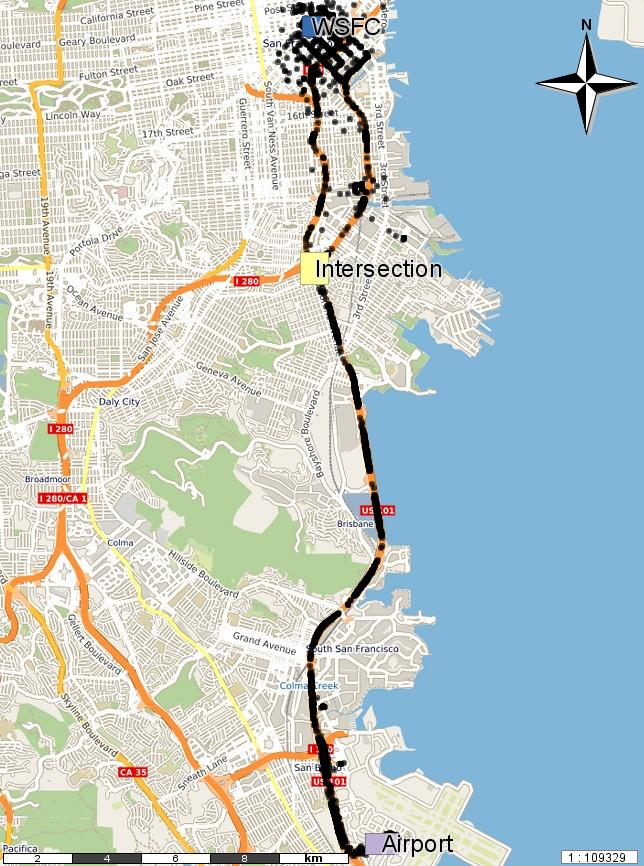
\includegraphics[width=.49\textwidth]{Images/CRAWDAD-Trajectories-Painted}
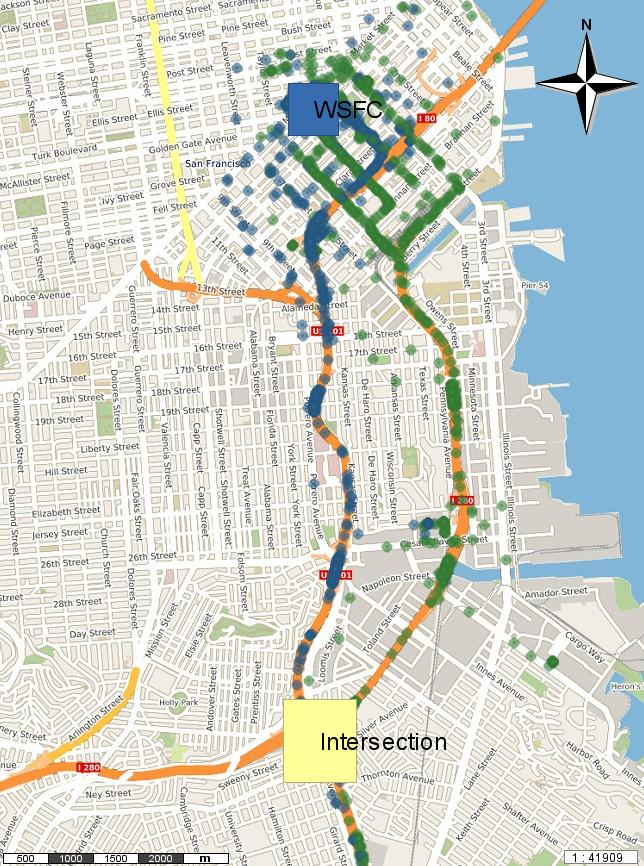
\includegraphics[width=.49\textwidth]{Images/CRAWDAD-Paths-Painted}
\caption{(left) \hl{taxi dataset} raw trajectories (right) \hl{taxi dataset raw trajectories represented with different colors, where blue points are the trajectories moving on highway 101 and green points being trajectories using highway 280}}
\label{fig:sanfrancisco_map_rois}
\end{figure}

With the objective of characterizing the trajectory movement, we separate the trajectories based on which road was used on the trip, whether 101 or 280, two major access roads \hl{from the south of the city to} WSFC. {Figure \ref{fig:sanfrancisco_map_rois}} (right) presents a zoom over trajectories moving on highways 101 (blue) and 280 (green) from Intersection to WSFC, where we can clearly visualize the different \hl{paths} that connect both regions.

Considering the stops WSFC, Intersection, and Airport, we consider as the ground truth the four distinct paths followed by the trajectories that move between these regions. These paths are shown in Table \ref{tab:san_francisco_dataset}. All 25 trajectories moving from Airport in direction to WSFC via highway 101 are defined as class A1. The 101 trajectories moving in opposite direction from WSFC to the Airport by highway 101 belong to class A2. The 34 trajectories moving from Airport in direction to WSFC by highway 280 belong to class B1 and the 44 trajectories moving from WSFC in direction to Airport by highway 280 belong to class B2. We assume that trajectories that belong to the same class should be more similar than trajectories of different classes.

\begin{table}[h]
\scriptsize
  \centering
  \begin{tabular}{|c|c|c|c|c|}
  	\hline
 Direction & Highway & Trajectories & Class \\
  	\hline
 Airport to WSFC & 101 & 25 & A1\\
 WSFC to Airport & 101 & 101 & A2\\
 Airport to WSFC & 280 & 34 & B1\\
 WSFC to Airport & 280 & 44 & B2\\
    \hline
  \end{tabular}
  \caption{Summary of trajectories extracted from the taxi trajectories dataset}
  \label{tab:san_francisco_dataset}
\end{table}

\subsubsection{Experimental evaluation}

In the following we describe the dimensions used to analyze the similarity of stops and moves. As spatial dimension of the stop we considered the centroid of the stop. As temporal dimension we used both start and end time of the stop, and as semantic information we used the name of the region (Airport, Intersection, and WSFC). For the moves, we use as spatial dimension the trajectory raw points of the move.

For measuring the similarity the following distance functions were considered for the stops.
\begin{itemize}
  \item Space: the Euclidean distance between the centroids of the stops:
	\item Time: let $[t1, t2]$ be a time interval of a stop, the time distance of two stops is given by the complement of the proportion between the intersection of their intervals and the total period between the minimum starting time and the maximum ending time of their intervals, as given in Equation \ref{eq:time_interval}
\begin{equation} \label{eq:time_interval}
	dist_t(a, b) = 1 - \dfrac{duration([a.t1, a.t2] \cap [b.t1, b.t2])}{duration([min(a.t1, b.t1), max(a.t2, b.t2)])}
\end{equation}
  \item Semantics: the distance is equal to 0 in case of exact match and equal to 1 otherwise
\end{itemize}

For the moves, we consider the following distance function:
\begin{itemize}
  \item Space: the spatial similarity of the moves is given by the UMS distance between the moves. We choose UMS because it is appropriate for low sampled trajectories, which is the case for this dataset, and it outperformed all existing similarity measures for raw trajectories evaluated in \cite{Furtado-UMS-2018}.
\end{itemize}

As several measures were not developed for semantic trajectories, for a more fair comparison we use existing measures over stops and over raw trajectories. For doing so we split the experiment in two parts: 1) a \textit{precision at recall} evaluation using only semantic trajectories; and 2) a \textit{precision at recall} evaluation using the raw trajectories. In (1) we run the experiment using the following measures: SMSM, MSM, MSTP, CVTI, LCSS and EDR. In (2) we run the experiment for the following measures: DTWa, wDF, LCSS, EDR and UMS.

Table {\ref{tab:san_francisco_measures}} presents the dimensions used in each measure. To general multidimensional similarity measures as MSM and MSTP, we provide as input all dimensions of each stop, namely: 1)  spatial information; 2) time interval; and 3) semantic information. We extend LCSS and EDR to support multiple dimensions, using the same strategy used in {\cite{Furtado:TGIS12156}}: given two multidimensional trajectories, two points are said as matched when all dimensions match, where each dimension has a distinct distance threshold. With those adaptations, both LCSS and EDR are used to measure similarity using the dimensions of space, time and semantics for stops. For CVTI, we provide as input the time interval of the stops and the stop names.

\begin{table}[!h]
\scriptsize
  \centering
  \begin{tabular}{|l|c|c|c|c|c|c|c|}
  	\hline
  & \multicolumn{4}{c|}{Semantic trajectories} & \multicolumn{2}{c|}{Raw trajectories} \\
 	\cline{2-5}
  & \multicolumn{3}{c|}{Stop} & \multicolumn{1}{c|}{Move} & \multicolumn{2}{c|}{} \\
 	\cline{2-7}
  & Space & Time & Semantic & Trajectory points & Space & Time\\
  	\hline
 SMSM & X & X & X & X & & \\
 MSM & X & X & X & & & \\
 DTWa &  &  &  & & X & X \\
 MSTP & X & X & X & & & \\
 CVTI & & X & X & & & \\
 wDF & & & & & X & \\
 UMS & & & & & X & \\
 LCSS & X & X & X & & X & X \\
 EDR & X & X & X & & X & X \\
    \hline
  \end{tabular}
  \caption{Dimensions used for each measure}
  \label{tab:san_francisco_measures}
\end{table}

Table \ref{tab:san_francisco_thresholds} shows the best thresholds used for measures that have thresholds. To define threshold values for the stops we experimented over a range of possible values of thresholds on each dimension (100m to 500m in a 100 meters step to stop spatial centroid distance and 0\% to 100\% in a 10 percentage points step to proportional stop time) and the best results obtained for each method were reported. For the move threshold the same approach was performed, varying the minimal distance for two moves match from 0 to 1 in a 0.1 unit step.

\begin{table}[!h]
\scriptsize
  \centering
  \begin{tabular}{|c|c|c|c|c|}
  	\hline
  & \multicolumn{3}{c|}{Semantic trajectories} & \multicolumn{1}{c|}{Raw trajectories} \\
 	\cline{2-5}
  & Space (meters) & Time proportion & Move & Space (meters) \\
  	\hline
 SMSM & 100 & 0.3 & 0.1 & - \\
 MSM & 100 & 0.3 & - & - \\
 MSTP & - & 0.8 & - & -  \\
 CVTI & - & 0.8 & - & -  \\
 LCSS & 100 & 0.3 & - & 100 \\
 EDR & 100 & 0.3 & - & 100 \\
    \hline
  \end{tabular}
  \caption{Thresholds used for each measure}
  \label{tab:san_francisco_thresholds}
\end{table}

\begin{figure*}[ht!]
\centering
\centerline{
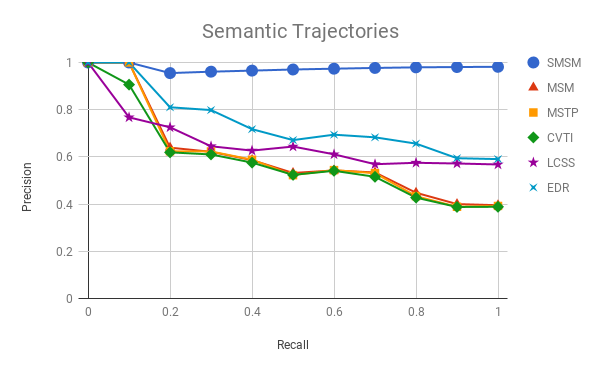
\includegraphics[width=0.5\textwidth]{Images/P_R-chart_San_Francisco.png}
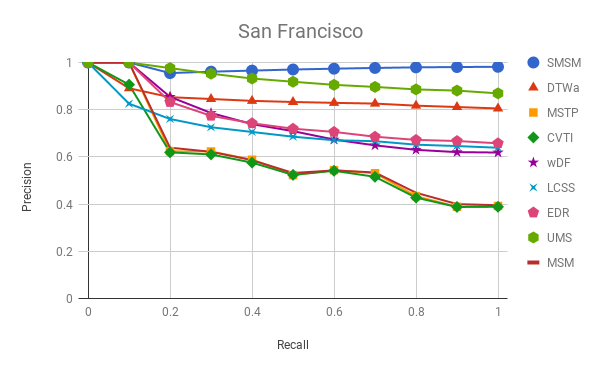
\includegraphics[width=0.5\textwidth]{Images/P_R-chart_San_Francisco-raw.png}
}
\caption{Precision at recall results for (left) semantic and (right) raw trajectories}
\label{fig:sanfrancisco_precision_recall}
\end{figure*}

\begin{table}[h]
\scriptsize
  \centering
  \begin{tabular}{|l|c|c|c|c|}
  	\hline
 & \multicolumn{2}{c}{Semantic} & \multicolumn{2}{|c|}{Raw} \\
 	\cline{2-5}
 & MAP & AUC & MAP & AUC \\
  	\hline
SMSM & \textbf{0.97} & \textbf{0.98} & - & -\\
MSM & 0.57 & 0.60 & - & -\\
DTWa & - & - & 0.84 & 0.87\\
MSTP & 0.56 & 0.60 & - & -\\
CVTI & 0.55 & 0.58 & - & -\\
 wDF & - & - & 0.73 & 0.75\\
LCSS & 0.65 & 0.67 & 0.55 & 0.57\\
 EDR & 0.72 & 0.74 & 0.64 & 0.66\\
UMS & - & - & 0.92 & 0.93 \\
    \hline
  \end{tabular}
  \caption{MAP and AUC evaluation for \hl{taxi} dataset}
  \label{tab:sanfrancisco_measures_map_auc}
\end{table}

Figure {\ref{fig:sanfrancisco_precision_recall}} presents the graphs with the results of the experiments on semantic and raw trajectories. As can be seen, SMSM out perform all other measures. Table {\ref{tab:sanfrancisco_measures_map_auc}} shows the MAP and AUC results for all measures, considering both semantic (Figure \ref{fig:sanfrancisco_precision_recall} left) and raw trajectories (Figure \ref{fig:sanfrancisco_precision_recall} right). The 1st and 2nd columns of Table {\ref{tab:sanfrancisco_measures_map_auc}} show that the results of SMSM(0.97/0.98) for MAP and AUC were significantly higher than MSM(0.57/0.60), MSTP(0.56/0.60), CVTI(0.55/0.58), LCSS(0.65/0.67) and EDR(0.72/0.74) considering semantic trajectories. The 3rd and 4th columns in Table {\ref{tab:sanfrancisco_measures_map_auc}} show the comparison of SMSM with approaches developed for raw trajectories. The results show that SMSM(0.97/0.98) still outperform the other measures, being DTWa(0.84/0.87), LCSS(0.55/0.57), EDR(0.64/0.66), wDF(0.73/0.75) and UMS(0.92/0.93) less accurate.

\hl{The \emph{precision at recall} results with semantic trajectories shown that SMSM is consistently better to recover the relevant trajectories than the other methods in all recall levels. The better results are explained by both the \emph{move} comparison and the sequence of the \emph{stops}. The next two most accurate measures were EDR and LCSS. Both measures remain the sequential characteristic of trajectory, but them demand the data to be homogeneous, and as we initially claimed that \emph{stops} and \emph{moves} are intrinsically heterogeneous, it does not be able to deal with both \emph{stop} and \emph{move} of the semantic trajectories. MSM also does not handle heterogeneous data and it does not take the sequence of elements into account either. This explains the poor results, since it ignores some important information about trajectory. CVTI and MSTP, despite of being LCSS-based measures, have the poorest results because them does not take into account some information, such as geospatial data in CVTI, or the use of only the frequency of the \emph{stops}, as in MSTP.

The \emph{precision at recall} results with raw trajectories also shown SMSM as better to recover the relevant trajectories in almost all recall levels. The second better results were UMS. UMS better results fall on it dynamic ellipses. The use of ellipses allows UMS to be more resilient over the low sampled trajectories. The third most accurate measure was DTWa. We can use the DTWa in this scenario because the data is composed by numeric values as latitude and longitude coordinates, the appropriate data type to DTWa. As DTWa tries to minimize the overall distance between two raw trajectories, the GPS points of the \emph{moves} help the measure to correctly recover the trajectories of the same class. EDR and LCSS measures, besides originally developed to raw trajectories, had poor results with raw trajectories. This occurs because of the low sampling rate in the data. As both measures compare trajectories point-by-point and they make the point match only when the distance of two points is less than a threshold, the smaller the sampling rate, the worse the result. wDF also compares trajectories point-by-point, but it \emph{window} parameter allows it to minimize the impact of low sampled trajectories. Because of this, wDF had better results than LCSS and EDR even being a point-to-point measure. Even so, the SMSM results with semantic trajectories were better than all other raw similarity measures.}

\subsection{Experiment with the Geolife Dataset}\label{sec:geolife}

The \textbf{Geolife} dataset is a well-known trajectory dataset, created by Microsoft Research Asia \citep{zheng2009mining} containing trajectories of 182 users, moving around Beijing, collected between April 2007 and August 2012. As a preprocessing step, we split trajectories when a 5 minutes gap between two consecutive points was found, since the trajectories of this dataset are highly sampled (lower than 2s).

\begin{figure}[ht!]
\centering
\centerline{
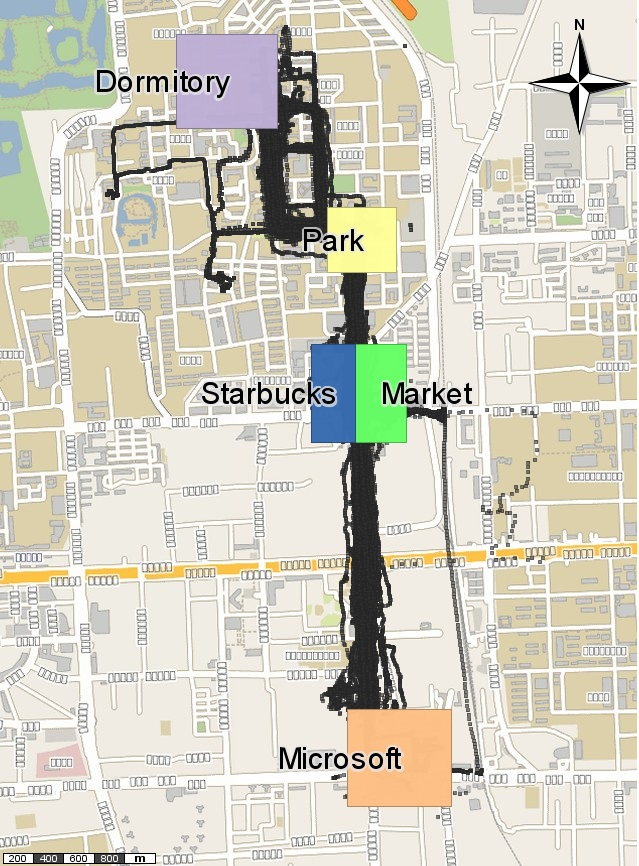
\includegraphics[width=.5\textwidth]{Images/Geolife-Trajectories-painted}
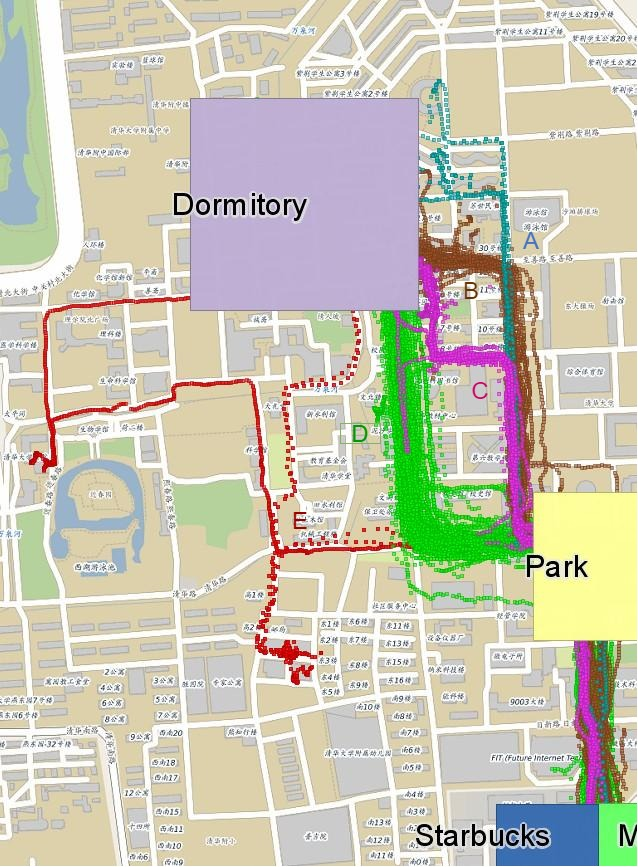
\includegraphics[width=.5\textwidth]{Images/Geolife-Paths-painted}
}
\caption{(left) trajectories moving between the regions Microsoft, Starbucks, Market, Park, and Dormitory (right) zoom over the distinct paths followed between Park and Dormitory}
\label{fig:geolife_map_rois}
\end{figure}

\subsubsection{Ground Truth Definition}
To build the ground truth, in this experiment we chose an area in Beijing, where pedestrians move between the University Dormitories and Microsoft Research Office. We considered five places as stops (Microsoft, Starbucks, Market, Park and Dormitory), that are show in Figure \ref{fig:geolife_map_rois} left. We considered 5 distinct paths connecting them, labeled as A, B, C, D, and E, as shown in Figure \ref{fig:geolife_map_rois} (right).

In Table \ref{tab:geolife_dataset} we define as ground truth 8 distinct classes of movement based on the sequence of stops and the followed path: Microsoft to Dormitory via Market and Park by path A with 5 trajectories named as class A, Microsoft to Dormitory via Market and Park by path B with 40 trajectories named as class B, Dormitory to Microsoft via Park and Starbucks by path C with 11 trajectories named as class C, Dormitory to Microsoft via Park and Starbucks by path D with 115 trajectories named as class D1, Dormitory to Microsoft via Park and Market by path D with 7 trajectories named as class D2, Microsoft to Dormitory via Market and Park by path D with 149 trajectories named as class D3, Microsoft to Dormitory via Starbucks and Park by path D with 6 trajectories named as class D4 and Microsoft to Dormitory via Market and Park by path E with 4 trajectories named as class E.

\begin{table}[ht!]
\scriptsize
  \centering
  \begin{tabular}{|c|c|c|c|}
  	\hline
 Direction & Path &  Trajectories & Class \\
  	\hline
Microsoft to Dormitory via Market and Park& A & 5 & A \\
Microsoft to Dormitory via Market and Park& B & 40&B \\
Dormitory to Microsoft via Park and Starbucks& C & 11&C \\
Dormitory to Microsoft via Park and Starbucks& D & 115&D1 \\
Dormitory to Microsoft via Park and Market& D & 7&D2 \\
Microsoft to Dormitory via Market and Park& D & 149&D3 \\
Microsoft to Dormitory via Starbucks and Park& D & 6&D4 \\
Microsoft to Dormitory via Market and Park& E & 4& E \\
    \hline
  \end{tabular}
  \caption{Classes representing distinct paths for the ground truth}
  \label{tab:geolife_dataset}
\end{table}

\subsubsection{Experimental evaluation}

Using a similar methodology used for the first experiment, we calculate the precision at recall for all 8 classes in our ground truth, comparing the SMSM results to the other measures. The dimensions used for stops are: a) space; and b) the region name (Dormitory, Park, Starbucks, Market and Microsoft). For the moves we used the raw points of the move. The time dimension was not taken into account because in this experiment we have classes with few trajectories.

We consider the following distance functions for the stops.
\begin{itemize}
  \item Space: the Euclidean distance between the centroids of the stops;
  \item Semantics: the distance is equal to 0 in case of exact match and equal to 1 otherwise
\end{itemize}

For the moves, we consider the following distance function:
\begin{itemize}
  \item Space: the spatial similarity of the moves is calculated using the DTW distance between the moves. In this dataset we use DTW for the spatial distance because the trajectory points are highly sampled, and UMS is not a good measure when points are highly sampled as in the Geolife dataset.
\end{itemize}

Table \ref{tab:geolife_thresholds} presents the thresholds used in this experiment for each measure. As on the \hl{taxi dataset} experiment, we defined the thresholds by running each experiment over a range of possible threshold values and the best results for each method were reported. For raw trajectories, we evaluated as threshold values 2, 4, 6, 8 and 10 meters because this dataset is highly sampled and is of pedestrian trajectories. The threshold for the move dimension was defined as follows: two moves are said to match if the DTW distance between them is less than the sum of the Euclidean distance of the moves.

\begin{table}[!h]
\scriptsize
  \centering
  \begin{tabular}{|c|c|c|}
  	\hline
  & \multicolumn{1}{c|}{Semantic trajectories} & \multicolumn{1}{c|}{Raw trajectories} \\
 	\cline{2-3}
  & Space (meters) & Space (meters) \\
  	\hline
 SMSM & 100 & - \\
 MSM & 100 & - \\
 LCSS & 100 & 4 \\
 EDR & 100 & 8 \\
    \hline
  \end{tabular}
  \caption{Thresholds used for each measure}
  \label{tab:geolife_thresholds}
\end{table}

Figure \ref{fig:geolife_precision_recall} (left) presents the precision at recall graph for this experiment. As can be observed, SMSM has the highest precision. Table \ref{tab:geolife_measures_map_auc} gives a better idea on the results. The 1st and 2nd columns of Table \ref{tab:geolife_measures_map_auc} show that SMSM results for MAP and AUC (0.95/0.95) were higher than MSM (0.74/0.75), LCSS (0.74/0.75), EDR (0.74/0.75), MSTP (0.50/0.53), and CVTI (0.53/0.57). In addition, executing the experiment using raw trajectories (3rd and 4rd columns in Table \ref{tab:geolife_measures_map_auc}), the results of DTWa (0.86/0.87), LCSS (0.79/0.80), EDR (0.71/0.73), wDF (0.57/0.60), and UMS (0.84/0.85) did not reach the good results of SMSM.

\hl{As in the taxi dataset experiment, SMSM had the better results over all other measures with the semantic trajectories. Again, LCSS and EDR had worse results than SMSM because this measures do not take into account the \emph{move} element between the \emph{stops}. The results were not worst because them take into account the sequence of \emph{stops}. Even without considering both the \emph{move} information and the sequence of \emph{stops}, MSM had a similar precision at recall curve. This occurs in this experiment because our \emph{stops} of same semantic overlaps each other, leaving MSM to consider the \emph{stop} similarity as strongly based on it spatial dimension. If the \emph{stops} occur in a more distinct spatial locations, but remaining it semantics, MSM would say as similar two \emph{stops} spatially near, but semantically distinct, affecting it precision at recall results. MSTP and CVTI, as LCSS-based measures with constraints, suffer from the same problems of previous experiment: i) CVTI do not take into account the spatial dimension, and in this dataset the semantic dimension in \emph{stops} are closely related to spatial dimension; and ii) MSTP makes use of the frequency of the \emph{stops}, and all trajectories in this dataset are short and non-repetitive trajectories, demanding the measure to use only the spatial data of each \emph{stop}.

The precision at recall results with raw trajectories shown that SMSM outperform all other measures in all recall levels. DTWa results shown that, differently from previous experiment, it has a great precision where the sampling rate of GPS is high. In the Geolife dataset, each point is collected every 2 seconds approximately. That high sampled trajectories make all it points closer to each other, leaving the DTWa to measure as similar trajectories that crossing each other, as the case in this dataset, with trajectories passing through Market sometimes crossing trajectories passing through Starbucks. If the person spent most of the time in Market, the fact of cross trajectories of people staying in Starbucks do the trajectory similarity be higher. The same occur with LCSS and EDR. The measure wDF had a poor result because of \emph{window} parameter, where in a high sampled scenario, makes the measure evaluate many neighbor points and our dataset has the cross trajectories (as already said), increasing the probability of a point find out a point in trajectories of other class closer than trajectories from same class. If we lowering the \emph{window} parameter, the wDF becomes more susceptible to outlier GPS points, since window of GPS points analyzed is smaller. UMS measure, the second most precise measure in previous experiment, was the fourth more precise measure. This result occurred because the high sampling rate. UMS was designed to handle with low sampled trajectories by creating it ellipses around points. In a high sampled scenario, it ellipses tends to be small, not overlapping the points of other trajectories of same class.}

\begin{figure*}[ht!]
\centerline{
\centering
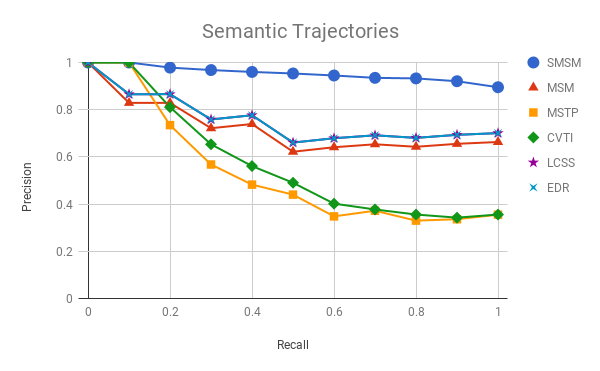
\includegraphics[width=.55\textwidth]{Images/P_R-chart_Geolife.png}
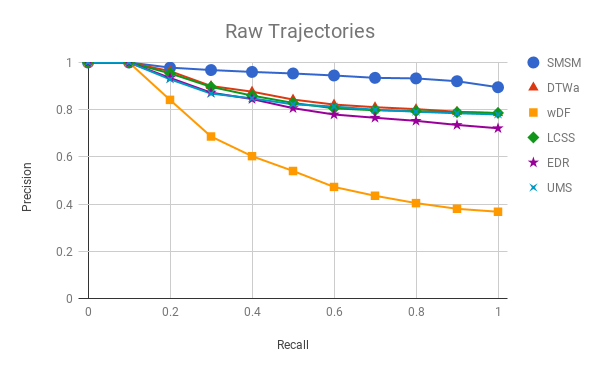
\includegraphics[width=.55\textwidth]{Images/P_R-chart_Geolife-raw.png}
}
\caption{Precision at recall results to semantic (left) and raw (right) trajectories}
\label{fig:geolife_precision_recall}
\end{figure*}

\begin{table}[ht!]
  \scriptsize
  \centering
  \begin{tabular}{|l|c|c|c|c|}
  	\hline
 & \multicolumn{2}{c}{Semantic}& \multicolumn{2}{|c|}{Raw}\\
 	\cline{2-5}
 & MAP & AUC& MAP & AUC\\
  	\hline
SMSM & \textbf{0.95} & \textbf{0.95} & - & -\\
 MSM & 0.74 & 0.75 & - & -\\
DTWa & - & - & 0.86 & 0.87\\
LCSS & 0.74 & 0.75 & 0.85 & 0.86\\
 EDR & 0.74 & 0.75 & 0.71 & 0.73\\
MSTP & 0.50 & 0.53 & - & -\\
CVTI & 0.53 & 0.57 & - & -\\
 wDF & - & - & 0.57 & 0.60\\
 UMS & - & - & 0.84 & 0.85\\
    \hline
  \end{tabular}
  \caption{MAP and AUC evaluation for the experiment with the Geolife dataset}
  \label{tab:geolife_measures_map_auc}
\end{table}

We notice that, in general, all similarity measures have a good result. However, we observed from the similarity scores that some measures having a high precision at recall, give a low similarity degree for trajectories of the same class that are highly similar. So to compare how well a measure can identify very similar trajectories of the same class, we perform another analysis: we extracted the mean similarity scores by class for each measure. We expect  all trajectories of the same class to be more similar between them, with higher similarity scores.
Table \ref{tab:geolife_similaritymeans} shows the mean similarity scores by class for each measure. For each measure, we choose the best AUC score, either from the semantic or raw trajectory results. The best results by class are in bold and the second better results are in italic. The results clearly show that the similarity score between trajectories of the same class is greater using SMSM than all others measures. The other two better measures in this analysis can be said to be MSM and DTWa. LCSS, for instance, had a good result in precision at recall in Table \ref{tab:geolife_measures_map_auc}, but the average similarity show in Table \ref{tab:geolife_similaritymeans} was the second worst measure, showing that LCSS similarity is dominated by low matching scores.

\begin{table}[ht!]
\footnotesize
  \centering
  \begin{tabular}{|c|c|c|c|c|c|c|c|c|c|}
  	\hline
 Class & SMSM & MSM & DTWa & EDR & UMS & wDF & MSTP & LCSS & CVTI \\
  	\hline
 A & \textbf{0.87} & $0.61$ & \textit{0.62} & $ 0.59$ & $0.37$ & $0.20$& $0.26$ & $0.20$ & $0.15$  \\
 B & \textbf{0.69} & \textit{0.52} & $0.50$ & $ 0.41$ & $0.04$ & $0.05$& $0.03$ & $0.02$ & $0.01$ \\
 C & \textbf{0.88} & \textit{0.60} & $0.58$ & $ 0.46$ & $0.12$ & $0.11$& $0.09$ & $0.09$ & $0.05$ \\
D1 & \textbf{0.86} & $0.52$ & \textit{0.53} & $ 0.42$ & $0.08$ & $0.02$& $0.01$ & $0.01$ & $0.01$ \\
D2 & \textbf{0.76} & $0.59$ & \textit{0.60} & $ 0.55$ & $0.19$ & $0.14$& $0.14$ & $0.14$ & $0.06$ \\
D3 & \textbf{0.83} & \textit{0.51} & $0.51$ & $ 0.43$ & $0.08$ & $0.02$& $0.01$ & $0.01$ & $0.01$ \\
D4 & \textbf{0.78} & \textit{0.58} & $0.55$ & $ 0.53$ & $0.25$ & $0.22$& $0.20$ & $0.17$ & $0.12$ \\
E  & \textbf{1.00} & \textit{0.75} & $0.74$ & $ 0.71$ & $0.59$ & $0.38$& $0.45$ & $0.25$ & $0.25$ \\
    \hline
  \end{tabular}
  \caption{Mean similarities by class for each measure}
  \label{tab:geolife_similaritymeans}
\end{table}

In summary, what is shown in Table \ref{tab:geolife_similaritymeans} is that state-of-the-art measures give very low scores for multidimensional trajectories that follow very similar paths (same class).

\subsection{Parameter Analysis}\label{sec:sensitivity}
\hl{SMSM needs two important parameters: the \emph{weight} of importance of \emph{stops} and the \emph{weight} of importance of \emph{moves}, with both \emph{weights} complementing each other. In other words, the weight of \emph{stops} plus the weight of \emph{moves} must sum 1. 
%The decision of correct weights needs a sensitivity analysis about the problem analyzed and the used data.

To show the impact of change in these parameters, we perform the Geolife experiment changing the weight proportion between \emph{stops} and \emph{moves}.
Table {\ref{tab:sensibility_stopmove}} shows the MAP score results. The most accurate execution was when the weight of \emph{moves} is $0.25$, achieving a MAP score of $0.95$ (better than the previously shown results comparing with other measures). As can be seen, if the influence of \emph{moves} is ignored (\emph{moves} weight = 0) SMSM achieves a MAP score of $0.75$. Those scores are indicating a confusion between the similarity of the trajectories of distinct classes, because trajectories of one class are so much similar to trajectories of another class that all them seem the same. The MAP score reaches $0.75$ only because the SMSM also considers the sequence of elements, keeping apart some classes with opposite directions, as such as Microsoft-Dormitory trajectories separated of Dormitory-Microsoft trajectories.}

\begin{table}[ht!]
  \scriptsize
  \centering
  \begin{tabular}{|c|c|}
  	\hline
Move weight & MAP \\
  	\hline
1.00 &0.93\\
0.75 & 0.94\\
0.50 & 0.94\\
0.25 & \textbf{0.95}\\
0.00 & 0.74 \\
    \hline
  \end{tabular}
  \caption{The MAP score evaluation for the sensibility experiment of weights with the Geolife dataset}
  \label{tab:sensibility_stopmove}
\end{table}

\hl{We also perform a sensibility analysis about the impact of thresholds of the distance functions. We evaluate how the spatial and the \emph{move} distance thresholds impact over the mean average precision (MAP) in the Geolife dataset. We split this experiment in two distinct analyses: (i) we use several different spatial thresholds and measure the MAP score for each similarity measure that use the spatial threshold, varying from 50 meters to 2,000 meters; and ii) we use several distinct thresholds for the \emph{move} distance computed as the DTW distance between the \emph{moves}, ranging from 0.5x of the sum of \emph{moves} to 10x of the sum of \emph{moves}.}

\hl{Table {\ref{tab:sensibility_spatial_thresholds}} presents the MAP score for each similarity measure that use the spatial threshold. The most accurate execution was when the spatial threshold is set between 50 and 300 meters, achieving a MAP score of $0.95$. Even the spatial threshold is set to higher values as 2,000 meters (an enough distance to go from Market region to Park region), SMSM is robust to achieve better results than the other measures. MSM, LCSS, and EDR measures are more severely punished by bigger thresholds, because them do not take in account the \emph{move} between the stops.}

\begin{table}[ht!]
  \scriptsize
  \centering
  \begin{tabular}{|l|c|c|c|c|}
  	\hline
Threshold (meters) & SMSM & MSM & LCSS & EDR\\
  	\hline
50 & \textbf{0.95} & 0.74 & 0.74 & 0.74 \\
100 & 0.95 & 0.74 & 0.74 & 0.74 \\
300 & 0.95 & 0.74 & 0.74 & 0.74 \\
500 & 0.93 & 0.42 & 0.69 & 0.69 \\
1000 & 0.93 & 0.42 & 0.69 & 0.69 \\
2000 & 0.93 & 0.42 & 0.38 & 0.38 \\
    \hline
  \end{tabular}
  \caption{The MAP score for each measure using spatial threshold when the spatial threshold varies from 50 meters until 2,000 meters}
  \label{tab:sensibility_spatial_thresholds}
\end{table}

\hl{Table {\ref{tab:sensibility_movement_thresholds}} presents the MAP score when the \emph{move} threshold changes. The most accurate execution was when the \emph{move} similarity threshold is set to $2.5 x$, indicating two \emph{moves} are equal if the DTW distance between them is equal or lower than 2.5 times the sum of it movement length. Using this threshold, the SMSM achieves the MAP score of $0.99$. From the $5 x$ multiplier on, the \emph{move} threshold starts to confuse some of \emph{movement elements} in trajectories, since the DTW distance begins to be smaller than the sum of \emph{moves} length multiplied by the threshold.}


\begin{table}[ht!]
  \scriptsize
  \centering
  \begin{tabular}{|l|c|}
  	\hline
Max DTW distance & MAP\\
  	\hline
$0.5 x$ & 0.89 \\
$1 x$ & 0.95 \\
$2.5 x$ & \textbf{0.99} \\
$5 x$ & 0.97 \\
$7.5 x$ & 0.96 \\
$10 x$ & 0.93 \\
    \hline
  \end{tabular}
  \caption{The MAP score evaluation when the \emph{move} attribute threshold varies from 0.5 x to 10 x of the sum of \emph{moves} length}
  \label{tab:sensibility_movement_thresholds}
\end{table}

\section{Discussion}
%Defining a correct and useful semantic value to each \emph{stop} is a challenging task, because each scenario might demands an appropriate choice of the semantics. 
%We can take the example of a public transportation planning application. Create a new bus line in a region demands to know previously all bus stops in the neighborhood, which bus lines already cover the region, and which bus line stops on each bus stop. Aside that, it is important to know how much people live and use other transportation means, such as taxis, car-pooling systems, bike-share programs, etc. To enrich a trajectory with this kind of data, we can use a ontological framework as proposed by } \cite{fileto2013baquara}\hl{. The Baquara Ontological Framework can enrich the \emph{stops} in the stop and move model with any kind of context information, based on available linked data collections.} 

%Other important choice to be made when using the SMSM is the weights of \emph{stops} and \emph{moves}. In the experiment described in Section {\ref{sec:sensitivity}}, we demonstrated the impact of weights in the AUC score and the average intraclass similarity. It indicates that depending on the application scenario, the \emph{stops} and the \emph{moves} play a different importance role. Our experiments are performed in scenarios which the \emph{moves} play a role of distinguishing trajectories but it do not help to distinguish the \emph{stops} itself. It occurs because the \emph{stops} are only some stationary points with well defined semantics. In scenarios where the \emph{stops} occurs in more distinct spatial locations, as in a public transportation system or a traffic management system, it is expected that the \emph{moves} plays a important role to distinguish trajectories based on the semantic of the \emph{stops}.

%The distance function thresholds, used to define if two elements (whether \emph{stops} or \emph{moves}) do match in a dimension or not, affect directly the precision results. We presented in experiment of Section  {\ref{sec:sensitivity}} the impact of threshold changes over the Geolife dataset, a high sampled trajectory datatset. This versatility of SMSM plays a crucial role, because as SMSM is a match-based measure, the definition of a threshold value demands a sensitivity analysis of trajectory data. For example, in an indoor trajectory context, it is expected that the GPS points have some inaccuracies in it coordinate values. Here, the threshold for a match in \emph{moves} should be lower than a more precise outdoor context, because the ellipses (using the UMS distance function) tend to be larger and less accurate. The same kind of analysis should be made in \emph{stops} dimensions, such as spatial, temporal, and the semantics, since the semantic distance function may be something more complex than direct equal or not equal.
%\hl{
%The choice of similarity measure also depends of what kind of problem we faced. For example, a problem which both the sequence of \emph{stops} and the movement between them play a relevant role in class definition. In this kind of scenario, SMSM showed up a better similarity measure, even when compared with raw trajectory similarity measures. Another kind of scenario when SMSM is a better choice is when the sequence of \emph{stops} play a relevant role, but the movement between them do not. DTWa, LCSS, and EDR also compute the similarity taking the sequence in account but them do this forcing the sequence to match over the trajectory. On the other hand the SMSM computes the similarity of each \emph{movement element}, giving a higher similarity to two \emph{movement elements} even both occur in distinct positions in the trajectories. But, when neither the sequence of \emph{stops} nor the movement between them are important, the MSM showed up a better choice, since it is the only measure that does not force the sequence of elements.}

\subsection{Comparison of measures in relation to applications}
\textcolor{red}{There are several types of trajectories and several ways to obtain these data. Depending on how these data were generated and their format, different  trajectory analysis and mining methods will be needed, and so different similarity measures can be applied. For applications that use raw GPS data, as trajectories of taxis, buses, or cars, with the intend to detect, for instance, traffic conditions or traffic jams, the most appropriate measure is UMS. UMS outperformed all measures for raw trajectories, because it is robust to trajectories with different sampling rates or different distances between trajectory points (the case when a trajectory varies the speed in a city), because instead of using a radious around each trajectory point to find the similar trajectories in the spatial neighbourhood, it uses an ellipses between every two trajectory points, and the size of the ellipses is dinamically build based on the distance between two trajectory points.}

\textcolor{red}{For applications that use GPS trajectories annotated only with stops or where the moves are not important, or trajectories extracted from social media data, which are more sparse and that do not have moves, i.e, the places visited by the user, the best measure is MSM. MSM is useful in tourism applications with these types of data, for instance, where one is interested in finding users that visit the same places, at similar times, but where the order of the visits is not important. In tourism applications where the analyst wants to find similar tourist trajectories to either predict or to recommend the next place to be visited, MSM is not appropriate because it ignores the order. When the sequence of the visited places is important, even when the details about the moves are not, SMSM is more appropriate, because it considers the stop order.}

\textcolor{red}{For dealing with GPS trajectories enriched with both stops and moves, and the spatial, temporal or semantic characteristcs of the stops and the moves are important, SMSM is the most appropriate measure. In a tourism application where the tourist has a time constraint to visit a city, a sequence of visits can be recommended based on the similarity analysis of other tourists that visited the same city but considering the visited places and the moves between the stops, in order to estimate the duration of the different movements between the stops. SMSM is the best measure for traffic analysis where the objective is to compare the traffic along  different paths that connect two regions in a city.}

\textcolor{red}{It is important to emphasize that in applications where the spatial movement of the moves is important, i.e., the raw trajectory points, SMSM can use the UMS measure to evaluate the move similarity.}

\section{Conclusion} \label{sec:conclusions}
In this work we extended MSM to support both stops and moves and partial sequence matching. We call the proposed measure SMSM. To the best of our knowledge, SMSM is the first semantic trajectory similarity measure that deals with both stops and moves, and where both are heterogeneous elements. 
The proposed similarity measure is robust  to consider multiple dimensions of stops and moves. A move, for instance, can be represented as raw points, the traveled distance, the major direction, the names of streets, etc.

By allowing the definition of weight for stops, moves and dimensions, the measure is flexible to give more or less importance for specific parts of trajectories. On the other hand, this weights may be difficult to estimate from the user point of view, but if he has no knowledge about the domain, the best is to define the same weight for all elements.

We performed different experiments, using real data of distinct contexts, including taxi trajectories and pedestrian trajectories. By evaluating SMSM with an information retrieval approach, we show that SMSM was more accurate than other measures developed either for raw or semantic trajectories.

SMSM requires a full partial match between the start and end stop of two movement elements to evaluate the move. In future works we will study an extension of SMSM to evaluate the move in cases where the end stops of two movement elements do not have a full match.

\bibliographystyle{tfv}
\bibliography{sbc-template}

\end{document}
